% !TeX root = ..

\subsection{
  Ограничения координат точек врезки и точек выключения инструмента,
  обусловленные деформацией материала при врезке
}
\label{sect:1.3.1}

Этот тип ограничений связан с тем,
что для соблюдения технологии врезки любая точка врезки
$M_k$
должна лежать (как отмечалось выше)
на некотором ненулевом расстоянии от контура детали,
по которому движется инструмент.
При этом координаты точки врезки должны,
естественно, находиться вне областей,
занимаемых геометрическими образами других деталей с учетом припуска на рез.
Величины необходимых минимально допустимых расстояний
от контуров детали до точек врезки и точек выключения
инструмента определяются различными технологическими параметрами.
Другими словами, этот тип ограничений носит геометрический характер
и определяет геометрические области на раскройной карте,
в которых допустимо задавать точки врезки для формирования сегментов резки.

Для общей формализации этих ограничений обозначим через
$E_j^d$ эквидистанты замкнутых контуров $C_j$,
удаленные от них на величину $d$,
а через
$P_j^d$ двумерные геометрические объекты
(замкнутые точечные множества),
ограниченные этими эквидистантами:
$E_j^d = \partial P_j^d$,
$P_j^d \subset \mathbb R \times \mathbb R$.
При этом будем полагать,
что для внешних контуров деталей
$E_j^d$
является внешней эквидистантой,
а для внутренних -- внутренней.
Пусть $OUT$ -- конечное множество индексов внешних контуров деталей,
а $IN$ -- соответственно множество индексов внутренних контуров.
Обозначим  размерность этих множеств соответственно $l$ и $s$,
т. е.
$OUT = \{j_1, j_2, \,\dots, j_l\};
IN = \{q_1, q_2, \,\dots, q_s\}$
$(OUT \subseteq \overline{1,N};
IN \subset \overline{1,N})$.
Заметим, что если $l=N$
(все контуры являются внешними), то
$IN = \varnothing$
$(s = 0)$.
Пусть $d1$ -- минимально допустимое расстояние от контуров деталей до точек врезки,
тогда выбранные точки врезки для каждого сегмента резки должны удовлетворять следующим условиям:
\begin{equation}
  \forall k \in \overline{1,K}:
  M_k \in G_M,
  \text{где}\:
  G_M = \big(B \setminus \bigcup_{j\in OUT} P_j^{d1} \big)
  \cup
  \big( \bigcup_{q\in IN}P_q^{d1} \big)
  .
  \label{pierce-constraint}
\end{equation}

Как мы уже отмечали,
минимально допустимое расстояние от граничных контуров деталей
до точек врезки,
задаваемых на границе листа,
или подготовленных предварительно механическим способом,
может быть несколько меньше,
чем до точек врезки, получаемым стандартным <<прожиганием>> (пробивкой) материала листа.
Для таких особых точек врезки область $G_M$,
задаваемая условием (\ref{pierce-constraint}),
может быть расширена.
Это условие является необходимым, но не достаточным,
и для конкретных задач могут возникать дополнительные ограничения,
обусловленные технологическими особенностями резки,
о которых пойдет речь ниже.
В этих случаях, наоборот, область $G_M$
может быть существенно сокращена.

Аналогичное условию (\ref{pierce-constraint})
ограничение справедливо и для точек выключения инструмента:
\begin{equation}
  \forall k \in \overline{1,K}:
  M_k^* \in G_{M^*},
  \text{где}\:
  G_{M^*} = \big(B \setminus \bigcup_{j\in OUT} P_j^{d2} \big)
	\cup
  \big( \bigcup_{q\in IN}P_q^{d2} \big)
  ,
  \label{tool-off-constraint}
\end{equation}
где $d2$ -- минимально допустимое расстояние
от контуров деталей до точек выключения инструмента,
которое чаще всего меньше $d1$
и может, как отмечалось, быть и нулевым.

Пример допустимых областей
(\ref{pierce-constraint})
представлен на
рис.~\ref{pierce-area}.

\begin{figure}[H]
  \centering
  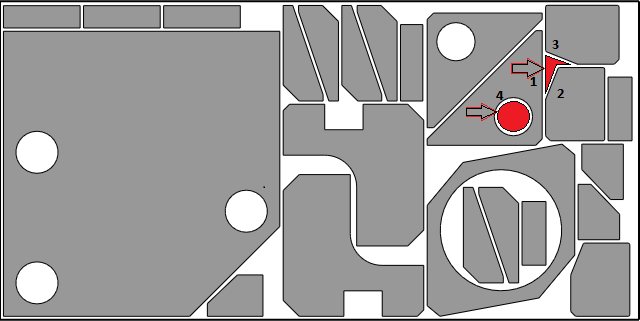
\includegraphics[width=0.9\textwidth]{pierce-area.png}
  \caption{
    Пример двух геометрических областей на раскройной карте
    (указаны~стрелками),
    допустимых для задания точек врезки
  }
  \label{pierce-area}
\end{figure}

Показаны две геометрические области листа,
одна -- определяемая
внешними граничными контурами деталей,
обозначенных на рисунке
\textit{1,2} и \textit{3},
и вторая --
внутренним граничным контуром
\textit{4}.
При этом минимально допустимое расстояние $d1$
от граничных контуров
\textit{1 -- 4} до возможных точек врезки,
установленное пользователем
\textit{CAM}-системы, равно 9,5 мм.
